%%%% Header %%%%%%%%%%%%%%%%%%%%%%%%%%%%%%%%%%%%%%%%%%%%%%%%%%%%%%%%%%%%%%%%%%%

\documentclass[
  12pt
]{scrartcl}

\usepackage{jonas}

\bibliography{/home/jon/lucile/share/jowncloud/sci/refs/refs.bib}
\hyphenation{}

%%%% Meta data %%%%%%%%%%%%%%%%%%%%%%%%%%%%%%%%%%%%%%%%%%%%%%%%%%%%%%%%%%%%%%%%

\usepackage[
  pdfauthor   ={Jonas Schöley},
  pdftitle    ={The Human Mortality Explorer},
  pdfsubject  ={Interactive Visualization},
  pdfkeywords ={visualization, R, shiny, mortality, hmd, Lexis surfaces},
  pdfproducer =Latex,
  pdfcreator  =pdflatex
]{hyperref}

\title{The Human Mortality Explorer}
\subtitle{An Interactive Online Visualization of the Human Mortality Database}
\author{Jonas Schöley}

%%%% Titlepage %%%%%%%%%%%%%%%%%%%%%%%%%%%%%%%%%%%%%%%%%%%%%%%%%%%%%%%%%%%%%%%%

\begin{document}

\maketitle

\begin{abstract}
The \emph{Human Mortality Explorer} is an interactive web-page visualising the death rates of the Human Mortality Database. The tools allows users from all around the world to easily explore human mortality dynamics across space and time. Users select data subsets on a graphical user interface and are immediately presented with results in the form of Lexis surface plots (Heatmaps over period and age). Users can toggle between a visualization of the pure mortality rates, sex differences in mortality and country differences. The Human Mortality Explorer is build using modern technologies that facilitate the construction of interactive web-pages without expert knowledge on web-technologies.
\end{abstract}

%%%% Text %%%%%%%%%%%%%%%%%%%%%%%%%%%%%%%%%%%%%%%%%%%%%%%%%%%%%%%%%%%%%%%%%%%%%

\begin{figure}[ht!]
  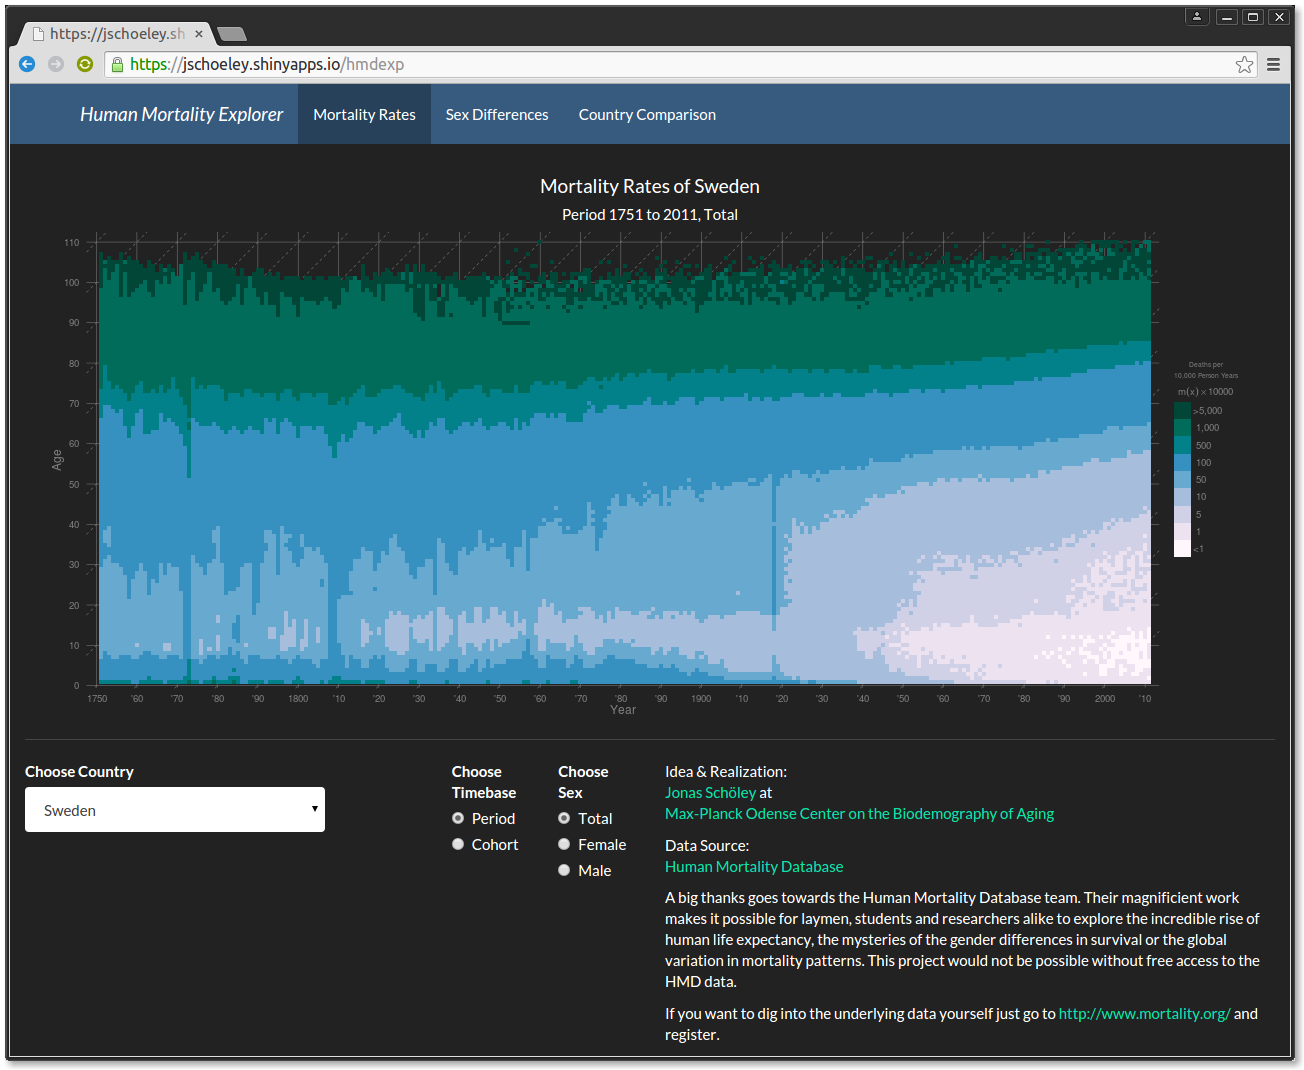
\includegraphics[width = \linewidth]{./fig/hmd_screen_mx.png}
  \caption{The Human Mortality Explorer: Mortality surface view.}
\end{figure}

\begin{figure}[ht!]
  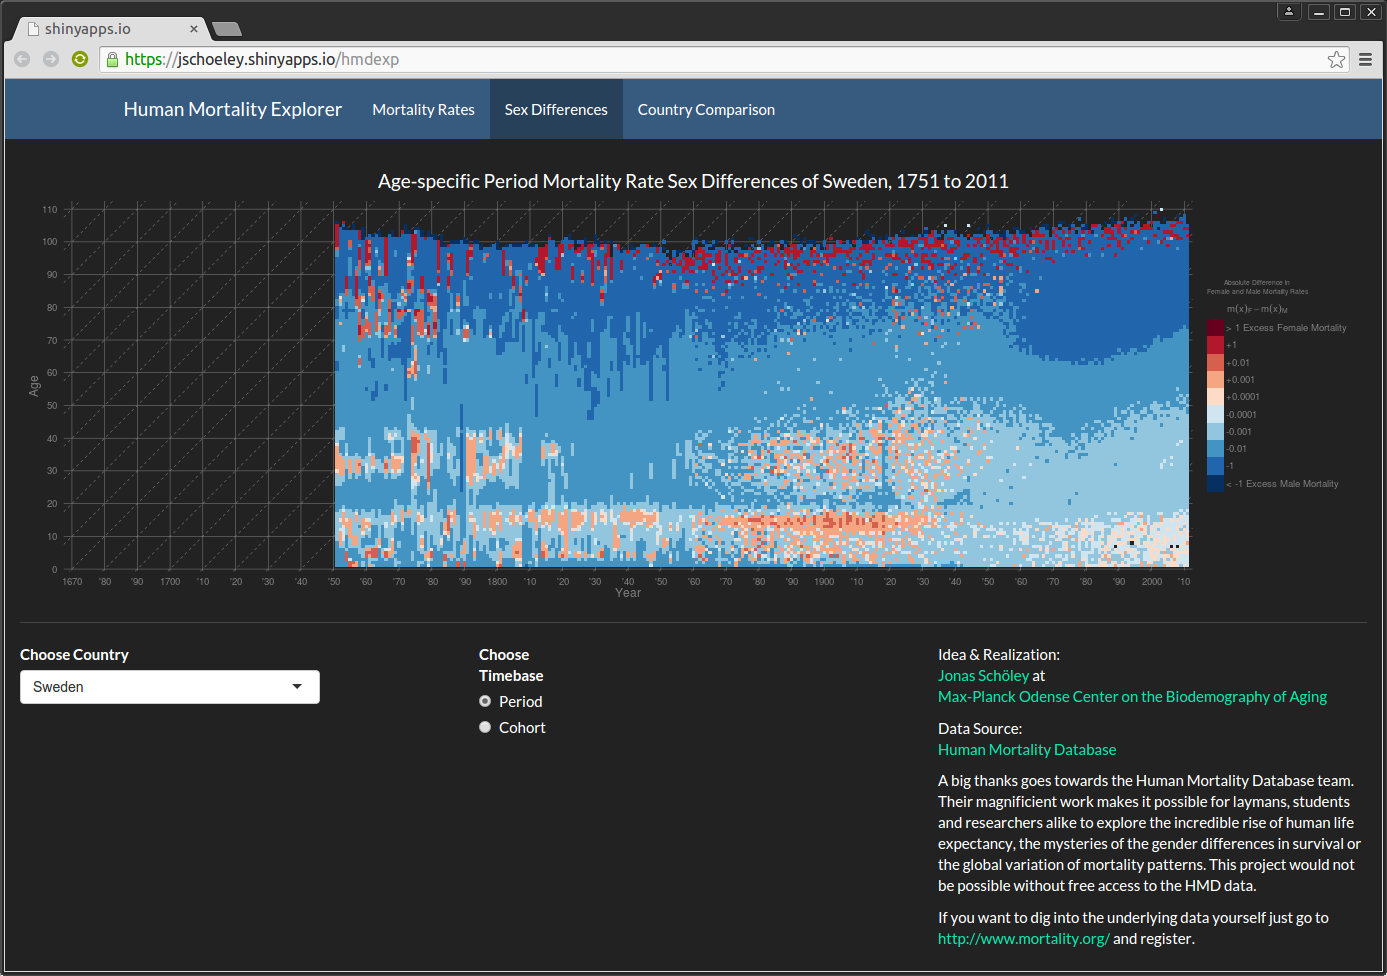
\includegraphics[width = \linewidth]{./fig/hmd_screen_mx_sex_diff.png}
  \caption{The Human Mortality Explorer: Sex differences view.}
\end{figure}

\begin{figure}[ht!]
  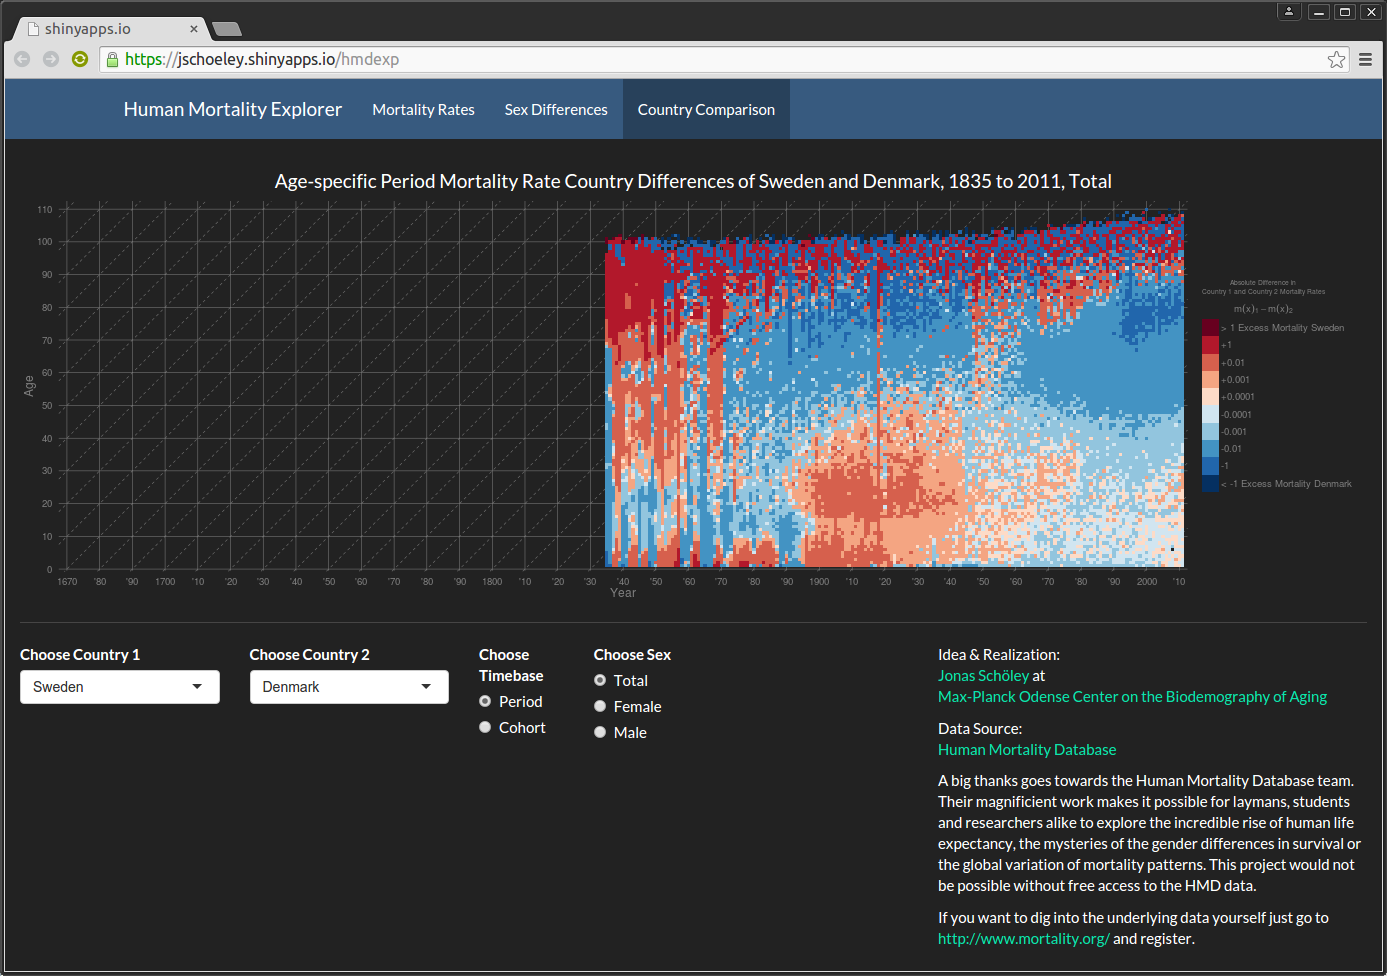
\includegraphics[width = \linewidth]{./fig/hmd_screen_mx_cntry_diff.png}
  \caption{The Human Mortality Explorer: Country comparison view.}
\end{figure}

The Human Mortality Explorer is in active development and not yet feature complete. Among other things, the final tool will allow for:

\begin{compactenum}
  \item The visualization of HMD life-table data ($d_x, q_x, l_x, L_x, T_x, e_x$),
  \item the selection of a continuous colour scale, and
  \item zooming into the graph.
\end{compactenum}

\clearpage

%%%% Bibliography %%%%%%%%%%%%%%%%%%%%%%%%%%%%%%%%%%%%%%%%%%%%%%%%%%%%%%%%%%%%%

\sloppy
\printbibliography

%\clearpage

%%%% Appendix %%%%%%%%%%%%%%%%%%%%%%%%%%%%%%%%%%%%%%%%%%%%%%%%%%%%%%%%%%%%%%%%%

% appendix figures follow A1, A2, B1... scheme
%\renewcommand\thefigure{\thesection.\arabic{figure}}
%\setcounter{figure}{0}

%\begin{appendix}
%\end{appendix}

\end{document}